\chapter{Schmale Flüsse mit Zurücksetzen}\label{chapter-thin-flows}
\newcommand*{\PlH}{\makebox[1ex]{\textbf{$\cdot$}}}

\section{Definition und Eigenschaften}

Der Abschnitt beginnt mit der Einführung einer neuen Klasse statischer Flüsse:

\begin{definition}[$s$-Netzwerk mit Zurücksetzen]
	Ein \emph{$s$-Netzwerk} ist ein azyklisches Netzwerk $(V, E, u)$, in dem alle Knoten von $s$ aus erreicht werden können.
	Ist ein Balancevektor $b\in\R^V$ gegeben, so erfüllt er $b_v\leq 0$ für alle $v\in V\setminus \{ s \}$.
	
 Stattet man ein $s$-Netzwerk mit einer Menge \emph{zurücksetzender Kanten $E_1\subseteq E$} aus, so heißt das Tupel $(V, E, u, b, s, E_1)$ ein \emph{$s$-Netzwerk mit Zurücksetzen auf $E_1$}.
\end{definition}

\todo{Irgendwie dieses Netzwerk am Anfang definieren}

\begin{definition}[Auslastung]
	Sei ein $b$-Fluss $f$ in einem $s$-Netzwerk mit Zurück\-setzen auf $E_1$ gegeben.
	Dann bezeichnet $f_e/u_e$ die \emph{Auslastung einer Kante $e$ durch $f$}.
	Die \emph{Auslastungsübertragung einer Kante $vw$} ist gegeben durch \[ \rho_{vw}(l_v, f_{vw}) \coloneq \begin{cases}
		\max\{ l_v, f_{vw} / u_{vw} \}, & \text{falls $vw\notin E_1$,}\\
		f_{vw} / u_{vw}, & \text{falls $vw\in E_1$.}
	\end{cases}
	\]
	Die \emph{Auslastung eines $s$-$v$-Pfades $P=(e_1,\dots,e_k)$} ist dann gegeben durch die Verkettung $\rho_{e_k}(\PlH, f_{e_k})\circ \dots \circ \rho_{e_1}(\PlH, f_{e_1})(0)$.
	Die zu $f$ \emph{zugehörige Knotenauslastung $l\in\R_{\geq 0}^V$} sei dann für einen Knoten $v\in V$ festgelegt durch die minimale Auslastung eines $s$-$v$-Pfades.
\end{definition}

Betrachtet man einen $s$-$v$-Pfad $P=(e_1, \dots, e_k)$, der Kanten aus $E_1$ enthält, so ist die Auslastung von $P$ gerade $\max_{j=i}^k f_{e_j}/u_{e_j}$, wobei $e_i$ die letzte Kante des Pfades in $E_1$ ist.
Daher nennt man die Kanten in $E_1$ die zurücksetzenden Kanten, da sie die Auslastung eines vorangegangen Pfades auf ihre eigene zurücksetzen.

\begin{proposition}\label{prop-congestion-labels-dijkstra}
	Die Knotenauslastungen eines $b$-Flusses $f$ in einem $s$-Netzwerk mit Zurücksetzen auf $E_1$ sind gegeben durch die eindeutige Lösung $(\tilde{l}_v)_{v\in V}$ des Gleichungssystems
	\[
	\tilde{l}_w = \begin{cases}
		0, & \text{falls $w=s$,}\\
		\min_{vw\in \delta^-(w)} \rho_{vw}(\tilde{l}_v, f_{vw}), & \text{sonst.}
	\end{cases}
	\]
\end{proposition}
\begin{proof}
	Die Existenz einer Lösung folgt aus der Azyklizität des Netzwerks und wegen der Erreichbarkeit jedes Knotens von $s$ aus.
	
	Sei also $\tilde{l}\in\R_{\geq 0}^V$ die Lösung des Gleichungssystems.
	Der Teilgraph $(V, E')$ mit \[
	E'\coloneq \left\{ vw\in E ~\middle\vert~ \rho_{vw}(\tilde{l}_v, f_{vw}) = \min_{uw\in\delta^-(w)} \rho_{uw}(\tilde{l}_u, f_{uw}) \right\}
	\]
	ebenfalls azyklisch und jeder Knoten ist von $s$ aus erreichbar.
	Man zeige $l_w = \tilde{l}_w$ durch eine Induktion über die Distanz von $s$ zu $w$ bezüglich der Anzahl an Kanten.
	Für $w=s$ gilt offenbar $l_s = 0$.
	Sei nun ein $s$-$w$-Pfad $P$ gegeben, seien $vw$ die letzte Kante und $Q$ das restliche Anfangsstück dieses Pfades.
	Nach Induktionsvoraussetzung ist die Auslastung von $Q$ mindestens $\tilde{l}_v$.
	Daher ist die Auslastung von $P$ mindestens $\rho_{vw}(\tilde{l}_v, f_{vw})$ aufgrund der Monotonie von $\rho_{vw}(\PlH, f_{vw})$, wodurch $l_v \geq \tilde{l}_v$ folgt.
	Außerdem hat ein $s$-$v$-Pfad $P$, der in $(V, E')$ verläuft, Auslastung $\tilde{l}_v$.
	Da solch ein Pfad existiert, gilt also $l_v \leq \tilde{l}_v$.
\end{proof}

\newcommand{\problemThinFlow}{\textsc{ThinFlow}}
\begin{definition}[Schmaler Fluss]
	Seien ein $b$-Fluss $f$ in einem $s$-Netzwerk mit Zurück\-setzen auf $E_1$ sowie die durch $f$ induzierten Knotenauslastungen $l$ gegeben.
	Der Fluss $f$ heißt \emph{schmaler Fluss mit Zurücksetzen auf $E_1$}, falls die Auslastung jedes $s$-$v$-Pfades mit positivem Fluss $l_v$ beträgt.
	
	Existiert ein $b$-Fluss, so nennt man $(V, E, u, s, b, E_1)$ eine \emph{Instanz von $\problemThinFlow$}.
\end{definition}

Insbesondere ist bei einem schmalen Fluss die Knotenauslastung $l_v$ eines Knotens $v$ gerade die Auslastung eines jeden $s$-$v$-Pfades mit positivem Fluss und $0$, falls kein solcher existiert.

\begin{remark}
	Ronald Koch betrachtet in~\cite{Koch2012} allgemeinere schmale Flüsse: Dort ist das zugrundeliegende Netzwerk nicht als azyklisch vorausgesetzt.
	Diese Einschränkung wird hier im Sinne von~\cite{Cominetti2015} beibehalten.
\end{remark}

\begin{figure}
	\centering
	\newcommand{\newnode}[4]{\node[lul] (#1) at #2 {#3 \\[0.5em] #4};}
	\begin{subfigure}{\textwidth}
		\begin{tikzpicture}[lul/.style={draw,
			ellipse,
			align=center,
			inner sep=0pt,
			outer sep=4pt,
			text width=7mm,
			minimum height=1.5cm
		}]
		
		\newnode{0}{(0,2)}{$a$}{$32$}
		\newnode{1}{(3,2)}{$b$}{$0$}
		\newnode{2}{(5,0)}{$c$}{$-2$}
		\newnode{3}{(7,2)}{$d$}{$-12$}
		\newnode{4}{(10,3)}{$e$}{$-2$}
		\newnode{5}{(10,1)}{$f$}{$0$}
		\newnode{6}{(13,2)}{$g$}{$-16$}
		
		\begin{scope}[-Latex]
		\path [-Latex] (0) edge node[above] {$4$} (1);
		\path [-Latex] (0) edge[bend right] node[above right] {$4$} (2);
		\path [-Latex] (0) edge[bend left] node[above] {$4$} (4);
		\path [-Latex] (1) edge node[above right] {$2$} (2);
		\path [-Latex] (1) edge node[above] {$2$} (3);
		\path [-Latex] (2) edge node[above left] {$2$} (3);
		\path [-Latex] (3) edge node[above] {$1$} (4);
		\path [-Latex] (3) edge node[above] {$2$} (5);
		\path [-Latex] (4) edge node[above] {$1$} (6);
		\path [-Latex] (5) edge node[above] {$1$} (6);
		\end{scope}
		\end{tikzpicture}
		\subcaption{Das Netzwerk. Die Kanten $e$ sind mit Kapazitäten $u_e$ und die Knoten $v$ mit einem Bezeichner $v$ und einer Balance $b_v$ beschriftet.}
		\label{subfig-thin-flow-example-network}
	\end{subfigure}
	\par\bigskip
	\begin{subfigure}{\textwidth}
		\begin{tikzpicture}[lul/.style={draw,
			ellipse,
			align=center,
			inner sep=0pt,
			outer sep=4pt,
			text width=7mm,
			minimum height=1.5cm
		}]
		
		\newnode{0}{(0,2)}{$a$}{$0$}
		\newnode{1}{(3,2)}{$b$}{$2{,}75$}
		\newnode{2}{(5,0)}{$c$}{$2{,}75$}
		\newnode{3}{(7,2)}{$d$}{$5$}
		\newnode{4}{(10,3)}{$e$}{$2{,}5$}
		\newnode{5}{(10,1)}{$f$}{$5$}
		\newnode{6}{(13,2)}{$g$}{$8$}
		
		\begin{scope}[-Latex]
		\path [-Latex] (0) edge node[above] {$11/4$} (1);
		\path [-Latex] (0) edge[bend right] node[above right] {$11/4$} (2);
		\path [-Latex] (0) edge[bend left] node[above] {$10/4$} (4);
		\path [-Latex] (1) edge node[above right] {$1/2$} (2);
		\path [-Latex] (1) edge node[above] {$10/2$} (3);
		\path [-Latex] (2) edge node[above left] {$10/2$} (3);
		\path [-Latex] (3) edge node[above] {$0/1$} (4);
		\path [-Latex] (3) edge node[above] {$8/2$} (5);
		\path [-Latex] (4) edge node[above] {$8/1$} (6);
		\path [-Latex] (5) edge node[above] {$8/1$} (6);
		\end{scope}
		\end{tikzpicture}
		\subcaption{Ein schmaler Fluss $f$ ohne Zurücksetzen.}
		\label{subfig-thin-flow-without-resetting}
	\end{subfigure}
	\par\bigskip
	\begin{subfigure}{\textwidth}
		\begin{tikzpicture}[lul/.style={draw,
			ellipse,
			align=center,
			inner sep=0pt,
			outer sep=4pt,
			text width=7mm,
			minimum height=1.5cm
		},
		scale=1]
		
		\newnode{0}{(0,2)}{$a$}{$0$}
		\newnode{1}{(3,2)}{$b$}{$3$}
		\newnode{2}{(5,0)}{$c$}{$3$}
		\newnode{3}{(7,2)}{$d$}{$5{,}5$}
		\newnode{4}{(10,3)}{$e$}{$2$}
		\newnode{5}{(10,1)}{$f$}{$5{,}5$}
		\newnode{6}{(13,2)}{$g$}{$8$}
		
		\begin{scope}[-Latex]
		\path [-Latex] (0) edge node[above] {$12/4$} (1);
		\path [-Latex] (0) edge[bend right] node[above right] {$12/4$} (2);
		\path [-Latex] (0) edge[bend left] node[above] {$8/4$} (4);
		\path [-Latex] (1) edge node[above right] {$1/2$} (2);
		\path [-Latex] (1) edge node[above] {$11/2$} (3);
		\path [-Latex] (2) edge node[above left] {$11/2$} (3);
		\path [Square-Latex] (3) edge node[above] {$2/1$} (4);
		\path [-Latex] (3) edge node[above] {$8/2$} (5);
		\path [-Latex] (4) edge node[above] {$8/1$} (6);
		\path [-Latex] (5) edge node[above] {$8/1$} (6);
		\end{scope}
		\end{tikzpicture}
		\subcaption{Ein schmaler Fluss mit Zurücksetzen auf $(d,e)$.}
		\label{subfig-thin-flow-with-resetting}
	\end{subfigure}
	\caption{Ein schmaler Fluss einmal ohne Zurücksetzen und einmal mit Zurücksetzen auf $(d,e)$.
		In den Abbildungen~\ref{subfig-thin-flow-without-resetting} und~\ref{subfig-thin-flow-with-resetting} sind die Kanten mit der Auslastung der Form $x_e/u_e$ und die Knoten mit der Knotenauslastung beschriftet.}
	\label{figure-thin-flow-example}
\end{figure}

\begin{example}
	In Abbildung~\ref{figure-thin-flow-example} ist ein Beispiel eines schmalen Flusses abgebildet.
	Die Kapazitäten der Kanten und die Balancen der Knoten des Ursprungsnetzwerk sind dabei in Abbildung~\ref{subfig-thin-flow-example-network} zu erkennen.
	Hervorzuheben ist, dass die Knoten $g$ mit Wert $16$ die größte und $d$ mit Wert $12$ die zweitgrößte Nachfrage haben.
	Außerdem haben die beiden einzigen Kanten $(e,g)$ und $(f,g)$, die zu $g$ führen, nur eine Kapazität von $1$.
	
	Betrachtet man zunächst den Fall ohne zurücksetzende Kanten, so stellt man fest, dass ein zugehöriger schmaler Fluss $x$ wie in Abbildung~\ref{subfig-thin-flow-without-resetting} diese beiden Kanten gleichmäßig auslasten muss:
	Die Auslastungen aller flusstragenden $a$-$g$-Pfade, egal ob sie über $e$ oder über $f$ zu $g$ gelangen, müssen in einem schmalen Fluss übereinstimmen.
	Aufgrund der hohen Nachfrage von $g$ und der geringen Kapazität seiner eingehenden Kanten, bestimmen diese letzten beiden Kanten die Auslastung jedes $a$-$g$-Pfades.
	
	Außerdem fällt auf, dass die Kante $(d,e)$ nicht genutzt wird.
	Auch das ist nicht besonders verwunderlich:
	Würde man Fluss von der Kante $(a, e)$ entfernen und stattdessen entlang eines Pfads $P$ über $d$ zu $e$ schicken, so hätte $P$ eine Auslastung von mindestens $5$, da jeder Pfad nach $d$ bereits Auslastung $5$ hatte.
	Weil aber $e$ aufgrund der Kante $(a,e)$ eine kleiner Auslastung als $2{,}5$ hat, kann der entstehende Fluss kein schmaler Fluss sein.
	Später in diesem Kapitel sehen wir, dass eine Kante, die zu einem Knoten niedrigerer Auslastung führt, in keinem schmalen Fluss ohne Zurücksetzen genutzt wird.
	
	Setzt man jedoch die Kante $(d, e)$ als zurücksetzende Kante voraus, so ist der Fluss aus Abbildung~\ref{subfig-thin-flow-without-resetting} kein schmaler Fluss auf dieser Instanz:
	Ein Pfad, der über $d$ nach $e$ verläuft, hat darin Auslastung $0$, da die letzte Kante des Pfades die Auslastung auf die eigene, also auf $0$, zurücksetzt.
	Insbesondere hat $e$ eine Auslastung von $0$, jedoch hat der $a$-$e$-Pfad $(a, e)$ Auslastung $2{,}5$, sodass es sich nicht um einen schmalen Fluss handeln kann.
	Ein schmaler Fluss mit Zurücksetzen auf $(d, e)$ schickt dagegen -- wie in Abbildung~\ref{subfig-thin-flow-with-resetting} zu sehen -- $2$ Flusseinheiten über $d$ zu $e$, sodass $e$ wie die Kante $(a,e)$ Auslastung $2$ hat.
\end{example}

\begin{lemma}\label{lemma-thin-flow-t-def}
	Ein $b$-Fluss $f$ in einem $s$-Netzwerk mit Zurücksetzen auf $E_1$ ist genau dann ein schmaler Fluss mit Zurücksetzen auf $E_1$, wenn eine Knotenbewertung $l\in\R_{\geq 0}^V$ existiert, die die folgenden Bedingungen erfüllt:
	\begin{enumerate}[label=(T\arabic*)]
		\item\label{def-thin-flow-source} $\displaystyle l_s = 0$,
		\item\label{def-thin-flow-x-zero} $\displaystyle l_w \leq l_v$, \tabto{4.5cm} für $vw\in E \setminus E_1$ mit $f_{vw}=0$,
		\item\label{def-thin-flow-x-positive} $\displaystyle l_w = \max\left\{ l_v, \frac{f_{vw}}{u_{vw}} \right\}$, \tabto{4.5cm} für $vw\in E\setminus E_1$ mit $f_{vw} > 0$,
		\item\label{def-thin-flow-resetting-edge} $\displaystyle l_w = \frac{f_{vw}}{u_{vw}}$, \tabto{4.5cm} für $vw\in E_1$,
		\item\label{def-thin-flow-no-resetting-edge} $\displaystyle l_w \geq \min_{vw\in \delta^-(w)} l_v$, \tabto{4.5cm} für $w\in V\setminus \{ s \}$ mit $\delta^-(w)\cap E_1 = \emptyset$.
	\end{enumerate}
	Diese Knotenbewertung stimmt dann mit der Knotenauslastung von $f$ überein.
	Außerdem gelten die Bedingungen~\ref{def-thin-flow-source}, \ref{def-thin-flow-x-zero} und~\ref{def-thin-flow-no-resetting-edge} bereits für die Knotenauslastungen von $f$, falls $f$ ein beliebiger $b$-Fluss ist.
\end{lemma}
\begin{proof}
	Sei $f$ ein schmaler Fluss mit Zurücksetzen auf $E_1$ und sei $l\in\R_{\geq 0}^V$ die Knotenauslastung von $f$.
	Man zeige, dass $l$ die Bedingungen~\ref{def-thin-flow-source}-\ref{def-thin-flow-no-resetting-edge} erfüllt, und benutze dabei die Darstellung aus Proposition~\ref{prop-congestion-labels-dijkstra}.
	Wegen $l_s = 0$ gilt bereits~\ref{def-thin-flow-source}.
	Für eine Kante $vw\in E\setminus E_1$ mit $f_{vw}=0$ gilt $l_w\leq \rho_{vw}(l_v, f_{vw}) = l_v$, wodurch auch~\ref{def-thin-flow-x-zero} folgt.
	Ist $vw\in E$ mit $f_{vw} > 0$, so existiert ein $s$-$w$-Pfad mit positivem Fluss, der die Kante $vw$ benutzt, sodass die Auslastung dieses Pfades $l_w=\rho_{vw}(l_v, f_{vw})$ ist, da der $s$-$v$-Teilpfad die Auslastung $l_v$ besitzt.
	
	Für $vw\notin E_1$ bedeutet das jedoch gerade $l_w = \max\{ l_v, f_{vw}/u_{vw} \}$, also~\ref{def-thin-flow-x-positive}, und für $vw\in E_1$ folgt $l_w = f_{vw} / u_{vw}$.
	Für~\ref{def-thin-flow-resetting-edge} bleibt der Fall $f_{vw} = 0$ zu prüfen:
	Hier gilt $l_w = \min_{uw\in\delta^-(w)} \rho_{uw}(l_u, f_{uw}) = f_{vw} / u_{vw} = 0$.
	Zuletzt betrachte man den Fall, dass $w\neq s$ keine eingehende zurücksetzende Kante hat.
	Da $w$ von $s$ aus erreichbar ist, hat $w$ mindestens eine eingehende Kante und dadurch folgt bereits $l_w = \min_{vw\in \delta^-(w)} \max\{ l_v, f_{vw} / u_{vw} \} \geq \min_{vw\in\delta^-(w)} l_v$, was auch~\ref{def-thin-flow-no-resetting-edge} impliziert.
	
	Sei nun umgekehrt $l\in\R_{\geq 0}^V$ eine Knotenbewertung, die~\ref{def-thin-flow-source}-\ref{def-thin-flow-no-resetting-edge} erfüllt.
	Man verwende eine Induktion über die Distanz eines Knotens $w$ zu $s$ bezüglich der Kantenzahl, um zu zeigen, dass $l_w$ die Knotenauslastung von $f$ ist.
	Für $w=s$ gilt $l_s=0$ bereits nach~\ref{def-thin-flow-source}.
	Für $w\neq s$ ist $l_w$ nach~\ref{def-thin-flow-x-zero},~\ref{def-thin-flow-x-positive} und~\ref{def-thin-flow-resetting-edge} eine untere Schranke an $\rho_{vw}(l_v, f_{vw})$ für $vw\in\delta^-(w)$.
	Es bleibt zu zeigen, dass für eine eingehende Kante $vw$ der Wert $\rho_{vw}(l_v, f_{vw})$ auch $l_w$ annimmt:
	Falls eine eingehende Kante $vw\in E_1$ oder eine eingehende Kante $vw$ mit $f_{vw} > 0$ existiert, ist $\rho_{vw}(l_v, f_{vw}) = l_w$ nach~\ref{def-thin-flow-resetting-edge} und~\ref{def-thin-flow-x-positive}.
	Sonst ist $l_w\geq \min_{vw\in \delta^-(w)} l_v = \min_{vw\in \delta^-(w)} \rho_{vw}(l_v, f_{vw})$ nach~\ref{def-thin-flow-no-resetting-edge}, was die Behauptung zeigt.
	Um zu sehen, dass $f$ nun ein schmaler Fluss mit Zurücksetzen auf $E_1$ ist, genügen die Bedingungen~\ref{def-thin-flow-source}, \ref{def-thin-flow-x-positive} und~\ref{def-thin-flow-resetting-edge}, da dadurch jeder $s$-$v$-Teilpfad eines Pfades mit positivem Fluss gerade Auslastung $l_v$ hat.
\end{proof}

\begin{remark}\label{remark-thin-flow}
	Hier ist, wie in~\cite[Definition~4]{Cominetti2011}, im Vergleich zu~\cite[Definition~6]{Koch2011} die Bedingung~\ref{def-thin-flow-no-resetting-edge} zusätzlich eingeführt worden.
	Diese ist nötig, um den Beweis von Theorem~\ref{thm-alpha-extension-is-nash-flow} zu geben, der in \cite{Koch2011} als Theorem~3 geführt wird.
	Dies wird in Bemerkung~\ref{remark-thin-flow-part-2} weiter erörtert.
	Die Änderung von $l_s=1$ auf $l_s=0$ wird später durch die Einführung normierter schmaler Flüsse in Definition~\ref{def-normalized-thin-flow} gerechtfertigt.
\end{remark}

\begin{lemma}\label{lemma-equivalent-thin-flow}
	In einer \problemThinFlow\ Instanz ist ein $b$-Fluss $f$ mit Knotenauslastung $l$ genau dann ein schmaler Fluss mit Zurück\-setzen auf $E_1$, wenn $f_{vw}= 0$ für alle Kanten $vw\in E$ mit $l_w < \rho_{vw}(l_v, f_{vw})$ gilt.
\end{lemma}
\begin{proof}
	Angenommen, $f$ sei ein schmaler Fluss mit Zurücksetzen auf $E_1$.
	Für eine Kante $vw\in E$ mit $l_w < \rho_{vw}(l_v, f_{vw})$ ist $vw\notin E_1$ und $f_{vw}=0$ nach~\ref{def-thin-flow-resetting-edge} und~\ref{def-thin-flow-x-positive}.

	Nun nehme man an, es gelte $f_{vw}=0$ für alle $vw\in E$ mit $l_w < \rho_{vw}(l_v, f_{vw})$, und man zeige die Eigenschaften~\ref{def-thin-flow-x-positive} und \ref{def-thin-flow-resetting-edge}.
	Der Rest folgt dann mit Lemma~\ref{lemma-thin-flow-t-def}.
	Ist $vw\notin E_1$ mit $f_{vw}>0$, so gilt $l_w = \rho_{vw}(l_v, f_{vw})$, wodurch Bedingung~\ref{def-thin-flow-x-positive} folgt.
	Für~\ref{def-thin-flow-resetting-edge} betrachte man zunächst Kanten $vw\in E_1$ mit $f_{vw}>0$:
	Hier folgt wieder $l_w = \rho_{vw}(l_v, f_{vw})$.
	Falls $f_{vw}=0$ gilt, ist $l_w=\min_{uw\in \delta^-(w)} \rho_{uw}(l_u, f_{uw}) = 0$.
\end{proof}

Mit anderen Worten: Eine Kante wird nur genutzt, falls die Auslastungs\-über\-tra\-gung durch die Kante gerade die Auslastung des Zielknotens ist.
Dies lässt sich folgern, da die Auslastungsübertragung nach Proposition~\ref{prop-congestion-labels-dijkstra} bereits eine untere Schranke an die Knotenauslastung ist.

\begin{lemma}[Eindeutigkeit der Knotenauslastung]\label{lemma-node-congestion-unique}
	Seien ein $s$-Netzwerk mit zurücksetzenden Kanten $E_1\subseteq E$ gegeben.
	Dann sind die Knotenauslastungen aller normierter schmaler Flüsse mit Zurücksetzen auf $E_1$ identisch.
\end{lemma}
\begin{proof}
	Angenommen, es existieren zwei normierte schmale Flüsse $f$ und $g$ mit Zurück\-setzen auf $E_1$ und unterschiedlichen Knotenauslastungen $l\neq h$.
	Dann ist ohne Beschränkung der Allgemeinheit die Menge $S\coloneq \{ v\in V \mid l_v > h_v \}$ nichtleer.
	Da $f$ und $g$ jeweils $b$-Flüsse sind, gilt 
	\begin{equation}\label{proof-uniqueness-labels-eq}
	f( \delta^+(S)) - f(\delta^-(S)) = b(S) = g(\delta^+(S)) - g(\delta^-(S)).
	\end{equation}
	Für aus $S$ herausgehende Kanten $vw\in \delta^+(S)$ gilt $f_e \leq g_e$, denn angenommen es gelte $f_e > g_e$, folgt mit Lemma~\ref{lemma-equivalent-thin-flow} und $v\in S$ die Ungleichung 
	\[l_w = \rho_{vw}(l_v, f_{vw}) > \rho_{vw}(h_v, g_{vw})\geq h_w,\]
	welche jedoch im Widerspruch zu $w\notin S$ steht.
	Ebenso gilt für Kanten $vw\in\delta^-(S)$ die Ungleichung $f_e \geq g_e$, weil sonst wegen $v\notin S$ die Ungleichung
	\[l_w \leq \rho_{vw}(l_v, f_{vw}) \leq \rho_{vw}(h_v, g_{vw}) = h_w\]
	gelten würde, was $w\in S$ widerspricht.
	Gleichung~\ref{proof-uniqueness-labels-eq} impliziert dann sogar $f_e = g_e$ für alle $e\in \delta(S)\coloneq \delta^-(S) \cup \delta^+(S)$.
	Für $vw\in \delta^-(S)$ ist dann $g_e=f_e=0$, da für $g_e=f_e>0$ wieder mit $v\notin S$ die Ungleichung $l_w = \rho_{vw}(l_v, f_{vw})\leq \rho_{vw}(h_v, g_{vw})=h_w$ der Bedingung $w\in S$ widerspricht.
	
	Aufgrund der Azyklizität existiert ein Knoten $w\in S$ mit $\delta^-(w)\subseteq \delta^-(S)$.
	Eingehende Kanten von $w$ sind daher nicht in $E_1$ enthalten, da für solch eine Kante $\rho_{vw}(l_v, f_e) = 0 = \rho_{vw}(l_v, g_e)$ gelten würde, sodass $l_w = 0 = h_w$ der Voraussetzung $w\in S$ widerspricht.
	Daher ist $l_w = \min_{vw\in \delta^-(w)} l_v$ und $h_w = \min_{vw\in\delta^-(w)} h_v$, was den Widerspruch $l_w \leq h_w$ impliziert.
\end{proof}

Zwar sind schmale Flüsse im Allgemeinen nicht eindeutig -- nichtmal ohne zurück\-setzende Kanten --, wie man leicht in Abbildung~\ref{figure-thin-flows-not-unique} erkennen kann, jedoch ist der Fluss auf einigen Kanten eindeutig:

\begin{figure}
	\centering
	\begin{subfigure}{.45\textwidth}
		\centering
		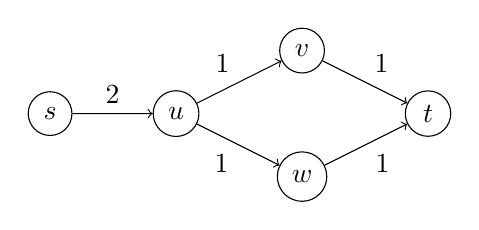
\begin{tikzpicture}[scale=0.8]
		\node[draw, circle] (S) at (0,2) {$s$};
		\node[draw, circle] (U) at (2,2) {$u$};
		\node[draw, circle] (W) at (4,1) {$w$};
		\node[draw, circle] (V) at (4,3) {$v$};
		\node[draw, circle] (T) at (6,2) {$t$};
		
		\path [->] (S) edge node[above] {$2$} (U);
		\path [->] (U) edge node[above left] {$1$} (V);
		\path [->] (U) edge node[below left] {$1$} (W);
		\path [->] (V) edge node[above right] {$1$} (T);
		\path [->] (W) edge node[below right] {$1$} (T);
		\end{tikzpicture}
	\end{subfigure}
	\begin{subfigure}{.45\textwidth}
		\centering
		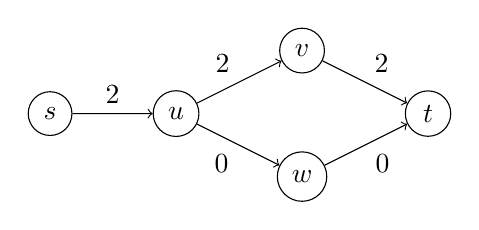
\begin{tikzpicture}[scale=0.8]
		\node[draw, circle] (S) at (0,2) {$s$};
		\node[draw, circle] (U) at (2,2) {$u$};
		\node[draw, circle] (W) at (4,1) {$w$};
		\node[draw, circle] (V) at (4,3) {$v$};
		\node[draw, circle] (T) at (6,2) {$t$};
		
		\path [->] (S) edge node[above] {$2$} (U);
		\path [->] (U) edge node[above left] {$2$} (V);
		\path [->] (U) edge node[below left] {$0$} (W);
		\path [->] (V) edge node[above right] {$2$} (T);
		\path [->] (W) edge node[below right] {$0$} (T);
		\end{tikzpicture}
	\end{subfigure}
	\caption{Zwei verschiedene schmale Flüsse derselben Instanz ohne Zurück\-setzen. Auf den Kanten steht der Flusswert; die Kapazitäten sind allesamt $1$.}
	\label{figure-thin-flows-not-unique}
\end{figure}

\begin{corollary}[Eindeutigkeit schmaler Flüsse]\label{corollary-thin-flows-uniqueness-on-some-edges}
	 Für eine Instanz von~$\problemThinFlow$ sind alle Lösungen auf den zurück\-setzen\-den Kanten sowie auf Kanten $vw$ mit $l_v \neq l_w$ identisch.
	 Dabei ist $(l_v)_{v\in V}$ die eindeutige Knotenauslastung.
\end{corollary}
\begin{proof}
	Da nach Lemma~\ref{lemma-node-congestion-unique} die Knotenauslastung $(l_v)_{v\in V}$ für jeden schmalen Fluss $f$ eindeutig ist, gilt $f_{vw} = u_{vw} l_w$ für zurücksetzende Kanten $vw$ nach~\ref{def-thin-flow-resetting-edge}.
	Für eine nicht-zurücksetzende Kante $vw\notin E_1$ betrachte man zunächst den Fall $l_v < l_w$.
	Nach Definition gilt $l_w \leq \max \{ l_v, f_{vw}/u_{vw} \}$, sodass man $f_{vw}/u_{vw} > l_v \geq 0$ folgern kann.
	Nach Lemma~\ref{lemma-equivalent-thin-flow} gilt also $f_{vw} = l_w u_{vw}$.
	Im Fall $l_v > l_w$ muss $f_{vw} = 0$ gelten, da sonst $l_w=\max\{ l_v, f_e/u_e \}$ gelten würde.
\end{proof}

\begin{theorem}\label{thm-existence-thin-flow}
	Für jede Instanz von $\problemThinFlow$ existiert ein schmaler Fluss.
\end{theorem}

Um die Existenz zu beweisen, benötigen wir zunächst den Fixpunktsatz von Kakutani.
Dazu führen wir die folgenden Begriffe ein:

\begin{definition}[Korrespondenz, Fixpunkt]
	Eine \emph{Korrespondenz} von einer Menge $A$ in eine Menge $B$ ist eine Abbildung $f: A \to \mathcal{P}(B)\setminus \{ \emptyset \}$ von $A$ in die Potenzmenge von $B$ ohne die leere Menge.
	Sind $A$ und $B$ topologische Räume, so nennt man $f$ \emph{abgeschlossen}, wenn die zugehörige Relation $R_f \coloneq \{ (a,b) \in A\times B \mid b\in f(a) \}$ in der Produkttopologie abgeschlossen ist.

	Ein \emph{Fixpunkt} einer Korrespondenz $f: X \to \mathcal{P}$ ist ein Punkt $x\in X$ mit $x\in f(x)$.
\end{definition}

Nun lautet der Fixpunktsatz von Kakutani (siehe~\cite{Heuser1991Fix}):

\begin{satz}[Fixpunktsatz von Kakutani]\label{satz-kakutani}
	Seien $C\subseteq E$ eine nichtleere, konvexe und kompakte Teilmenge eines normierten Raumes $E$ und $f: C \to \mathcal{P}(C)$ eine abgeschlossene, konvexwertige Korrespondenz.
	Dann besitzt $f$ einen Fixpunkt.
\end{satz}

\begin{proof}[Beweis von Theorem~\ref{thm-existence-thin-flow}]
	Man betrachte die Menge $C$ aller $b$-Flüsse als Teilmenge des metrischen Raums $\R^E$.
	Nach Voraussetzung ist diese nichtleer, konvex, da für $f, g\in C, \lambda \in [0,1]$ der Fluss $\lambda f + (1-\lambda)g$ wieder die Flusserhaltung erfüllt, und kompakt, da jeder Fluss in $C$ aufgrund der Azyklizität in $s$-$v_i$-Wege zerlegbar ist, wodurch jede Kante maximal Fluss $b_s$ besitzen kann, sodass $C$ eine beschränkte Teilmenge von $\subseteq [0, b_s]^E$ ist.
	Außerdem ist $C$ abgeschlossen, da es die Lösungsmenge eines linearen Gleichungssystem ist.
	Auf $C$ definiere man die Korrespondenz
	\[
	\Gamma: C\to \mathcal{P}(C)\setminus\{ \emptyset \}, ~ f\mapsto \{ g\in C \mid \forall vw\in E: l_w < \rho_{vw}(l_v, f_{vw}) \implies g_{vw} = 0 \}.
	\]
	Dabei sei $l\in\R_{\geq 0}^V$ die zu $f$ gehörige Knotenauslastung.
	Diese Korrespondenz ist wohldefiniert, da $\Gamma(f)$ für jedes $f\in C$ nichtleer ist:
	Der Knoten $s$ kann im Graphen $G'\coloneq (V, E')$ mit $E'\coloneq \{ vw\in E \mid \rho_{vw}(l_v, f_{vw})=l_w \}$ jeden Knoten erreichen, da $G'$ azyklisch ist und jeder Knoten $w\neq s$ mindestens eine eingehende Kante mit $l_w = \rho_{vw}(l_v, f_{vw})$ besitzt. 
	Daher existiert ein $s$-$v$-Weg $P_v$ in $G'$ für alle $v\in V$ und der Fluss $\sum_{v\in V\setminus\{ s\}} b_v \cdot P_v$ ist in $\Gamma(f)$ enthalten.
	
	Für jedes $f\in C$ ist $\Gamma(f)$ konvex: Ist für $g, h\in \Gamma(f), \lambda\in [0,1]$ und eine Kante $vw\in E$ die Bedingung $l_w < \rho_{vw}(l_w, f_{vw})$ erfüllt, so gilt auch $\lambda g_{vw} + (1-\lambda) h_{vw} = 0$, womit $\lambda g + (1-\lambda)h$ im Bild $\Gamma(f)$ liegt.
	Des Weiteren ist $\Gamma$ abgeschlossen: 
	Sei eine konvergente Folge $((f^{n}, g^{n}))_{n\in\N}$ in $R_\Gamma$ mit Grenzwert $(f, g)$ gegeben.
	Die zu $f$ bzw. $f^n$ gehörigen Knotenauslastungen seien gegeben durch $l$ bzw. $l^n$.
	Angenommen, es gelte $l_w < \rho_{vw}(l_v, f_{vw})$.
	Da die Zuordnung $f\mapsto l$ eines $b$-Flusses auf seine Knotenauslastung nach Lemma~\ref{prop-congestion-labels-dijkstra} stetig ist, existiert ein $N\in\N$ mit $l_w^n<\rho_{vw}(l_v^n, f_{vw}^n)$ für alle $n\geq N$.
	Damit ist auch $g_{vw} = \lim_{n\to\infty} g_{vw}^n = 0$.
	
	Daher existiert nach dem Fixpunktsatz von Kakutani~\ref{satz-kakutani} ein Fixpunkt von $\Gamma$, welcher nach Lemma~\ref{lemma-equivalent-thin-flow} ein schmaler Fluss mit Zurücksetzen auf $E_1$ ist.
\end{proof}

\section{Berechnung schmaler Flüsse}

Dieser Abschnitt diskutiert die Komplexität der Berechnung schmaler Flüsse.
Dazu schränken wir uns wie bei der Berechnung auslastungsminimaler Flüsse zunächst wieder auf solche mit rationalen Koeffizienten ein und erhalten das folgende Problem:

\newcommand{\probTFwR}{\textit{\textsc{(TFwR)}}}

\newcommand{\probTFwoR}{\textit{\textsc{(TFwoR)}}}

\begin{center}
	\begin{mdframed}
		\centering
		\emph{Thin Flow with Resetting \probTFwR} \\[1em]
		\begin{tabular}{rl}
			{\bfseries Input}: &\problemThinFlow\ Instanz $(V, E, u \in \Q^E_{>0}, s\in V, b\in \Q^V, E_1\subseteq E)$\\
			{\bfseries Output}: &Schmaler Fluss $f$ mit Zurücksetzen auf $E_1$
		\end{tabular}
	\end{mdframed}
\end{center}

Die Existenz schmaler Flüsse mit Zurücksetzen aus Theorem~\ref{thm-existence-thin-flow} suggeriert bereits einen exponentiellen Algorithmus, um einen solchen Fluss mit Wert $d$ zu berechnen:
Man rate die Menge $E'\subseteq E$ aller Kanten $vw$, die $l_w = \rho_{vw}(l_v, f_{vw})$ erfüllen sollen, sowie für alle $vw\in E'\setminus E_1$ eine Binärzahl $\sigma_{vw}\in\{0,1\}$, die $\max\{ l_v, f_{vw}/u_{vw}\} = \sigma_{vw} l_v + (1-\sigma_{vw}) f_{vw}/u_{vw}$ erfüllen soll.
Insbesondere sollen in $(V, E')$ immer noch alle Knoten von $s$ aus erreichbar sein.
Dann suche man einen zulässigen Punkt in folgendem Polyeder:
\begin{align*}
	& (f, l) \in \R_{\geq 0}^{E + V} \\[0.3em]
	\text{u.d.N.}\quad &
	f(\delta^+(v)) - f(\delta^-(v)) = b_v& \text{für $v\in V$,} \\[0.3em]
	& l_s = 0, \\[0.3em]
	&\mathopen{}\left.\begin{array}{@{}l}
		l_w = \sigma_{vw} l_v + (1-\sigma_{vw}) \frac{f_{vw}}{u_{vw}},\\[0.4em]
		\sigma_{vw} l_v + (1-\sigma_{vw}) \frac{f_{vw}}{u_{vw}} \geq \frac{f_{vw}}{u_{vw}},\\[0.4em]
		\sigma_{vw} l_v + (1-\sigma_{vw}) \frac{f_{vw}}{u_{vw}} \geq l_v,
	\end{array} \right\}\mathclose{}
	& \text{für $vw\in E'\setminus E_1$},\\[0.3em]
	& l_w = \frac{f_{vw}}{u_{vw}}, & \text{für $vw\in E_1$,} \\[0.3em]
	& \mathopen{}\left.\begin{array}{@{}l}
	f_{vw} = 0,\\[0.4em]
	l_w \leq l_v,
	\end{array} \right\}\mathclose{} & \text{für $vw\in E\setminus E'$.}
\end{align*}

Existiert solch ein Punkt $(f, l)$, so ist $f$ ein schmaler Fluss mit Zurücksetzen auf $E_1$ mit zugehöriger Knotenbewertung $l$:
Die Bedingung für Kanten $vw$ in $E'\setminus E_1$ lässt sich zusammenfassen zu $l_w = \max \{ l_v, f_{vw}/u_{vw} \}$.
Man prüfe die Bedingung aus Lemma~\ref{lemma-thin-flow-t-def}.
Dabei folgt~\ref{def-thin-flow-source} sofort.
Für Kanten $vw\in E\setminus E_1$ mit $f_{vw} = 0$ gilt $l_w \leq l_v$ mit Fallunterscheidung nach $vw\in E'$, also gilt~\ref{def-thin-flow-x-zero}.
Auch~\ref{def-thin-flow-x-positive} und~\ref{def-thin-flow-resetting-edge} folgen sofort.
Für~\ref{def-thin-flow-no-resetting-edge} nehme man also an, dass ein Knoten $w\neq s$ keine eingehenden Kanten in $E_1$ hat.
Da $w$ von $s$ aus in $(V, E')$ erreichbar ist, hat $w$ mindestens eine eingehende Kante $vw$ in $E'$, für die $l_w = \max\{ l_v, f_{vw}/u_{vw} \} \geq \min_{uw\in\delta^-(w)} l_u$ gilt.
Also ist auch~\ref{def-thin-flow-no-resetting-edge} erfüllt und $f$ ist ein schmaler Fluss mit Zurücksetzen auf $E_1$.

Setzt man andersherum für einen schmalen Fluss $f$ mit Knotenauslastung $l$ die Menge $E'$ als diejenigen Kante, die $l_w = \rho_{vw}(l_v, f_{vw})$ erfüllen, und $\sigma_{vw}$ als $1$, falls $l_v \geq f_{vw}/u_{vw}$ gilt, und sonst als $0$, so ist $(f, l)$ eine zulässiger Punkt im oben definierten Polyeder.
Dies kann leicht durch Heranziehen von Lemma~\ref{lemma-equivalent-thin-flow} eingesehen werden.

\newcommand{\TFNP}{\mathbf{TFNP}}

Die Zulässigkeit eines solchen Polyeders kann in polynomieller Zeit beispielsweise durch die Ellipsoidmethode \todo{add ref to search of rationals} ermittelt werden.
Da nach Theorem~\ref{thm-existence-thin-flow} für jede \problemThinFlow\ Instanz ein schmaler Fluss mit Zurücksetzen existiert, liegt das Problem \probTFwR\ in der Komplexitätsklasse $\TFNP$:

\begin{definition}[Suchproblem]
	Ein \emph{Suchproblem $\Pi$} ist eine Relation $\Pi\subseteq X \times Y$ zusammen mit der Problemstellung zu einer \emph{Instanz} $x\in X$ eine \emph{Lösung} $y\in Y$ mit $(x,y)\in \Pi$ zu ermitteln.
	
	Ein Suchproblem $\Pi\subseteq X\times Y$ heißt \emph{polynomiell reduzierbar} auf ein Suchproblem $\Pi'\subseteq X'\times Y'$, falls es zwei polynomiell berechnbare Funktionen $f: X\rightarrow X'$ und $g: Y\rightarrow Y'$ gibt, sodass $g(y)$ eine Lösung der Instanz $f(x)$ von $\Pi'$ für jede Lösung $y$ einer Instanz $x$ von $\Pi$ ist, d.h.
	\[ (x,y) \in \Pi \implies (f(x), g(y)) \in \Pi'.\]
\end{definition}
\begin{definition}[Komplexitätsklasse $\TFNP$]
	Ein Suchproblem $\Pi\subseteq X \times Y$ liegt genau dann in der Komplexitätsklasse $\TFNP$ (engl. Total Function Nondeterministic Polynomial), wenn es einen deterministischen, polynomiellen Algorithmus gibt, der entscheidet, ob $(x,y) \in \Pi$ für beliebige $x\in X$ und $y\in Y$ gilt, und wenn für alle $x\in X$ ein $y\in Y$ existiert, dessen Kodierung polynomielle Größe in der Kodierungslänge von $x$ besitzt, sodass $(x, y) \in \Pi$ gilt.
\end{definition}

In den folgenden Unterkapiteln soll diskutiert werden, ob es bessere Abschätzungen für die Komplexität von \probTFwR\ gibt.

\subsection{Berechnung schmaler Flüsse ohne Zurücksetzen}

Man betrachte zunächst einen Spezialfall des Problems:
Dabei soll es um die Bestimmung von schmalen Flüssen in Netzwerken ohne zurücksetzende Kanten gehen.
Daraus entsteht die folgende Problemformulierung:

\begin{center}
	\begin{mdframed}
		\centering
		\emph{Thin Flow without Resetting \probTFwoR} \\[1em]
		\begin{tabular}{rl}
			{\bfseries Input}: &\problemThinFlow\ Instanz $(V, E, u \in \Q^E_{>0}, s\in V, b\in \Q^V, E_1=\emptyset)$\\
			{\bfseries Output}: &Schmaler Fluss $f$ ohne Zurücksetzen
		\end{tabular}
	\end{mdframed}
\end{center}

In diesem Abschnitt wird ein polynomieller Algorithmus zur Berechnung von schmalen Flüssen ohne Zurücksetzen vorgestellt.
Dieser wurde~\cite{Koch2012} entnommen.
Dazu wird zunächst der Zusammenhang dieser Flüsse mit auslastungsminimalen Flüssen erarbeitet:

\begin{lemma}\label{lemma-thin-flows-without-resetting-have-minimal-congestion}
	Sei ein schmaler $b$-Fluss $f$ ohne Zurücksetzen mit zugehöriger Knotenauslastung $l$ gegeben.
	Dann ist $f$ ein $b$-Fluss minimaler Auslastung $q$ und für $E\neq\emptyset$ ist $X\coloneq \{ v\in V \mid l_v < q \}$ ein dünnster Schnitt.
\end{lemma}
\begin{proof}
	Ist $b$ der Nullvektor -- wie im Fall $E=\emptyset$ --, so ist $f$ der Nullfluss, da das Netzwerk azyklisch ist.
	
	Sei also $q>0$ die Auslastung von $f$ im Falle von $b\neq 0$.
	Nach Korollar~\ref{cor-easy-characterization-sparsest-cut} genügt es zu
	zeigen, dass die Auslastung jeder ausgehenden Kante von $X$ bezüglich $f$ gerade $q$ beträgt und auf eingehenden Kanten von $X$ kein Fluss fließt.
	Wegen $l_s=0$ ist $s$ im Schnitt $X$ enthalten.
	Sei $vw\in\delta^+(X)$ eine ausgehende Kante.
	Dann gilt $l_v < l_w = q $ und nach Proposition~\ref{prop-congestion-labels-dijkstra} auch $q = l_w \leq \rho_{vw}(l_v, f_{vw}) = f_{vw} / u_{vw}$.
	Da $q$ eine obere Schranke an $f_{vw}/u_{vw}$ ist, gilt also $f_{vw}/u_{vw} = q$.
	Für eine eingehende Kante $vw\in\delta^-(X)$ gilt $\rho_{vw}(l_v, f_{vw})\geq l_v > l_w$ und somit muss nach Lemma~\ref{lemma-equivalent-thin-flow} der Fluss $f$ auf der Kante $vw$ verschwinden.
\end{proof}

\begin{definition}
	Seien $\mathcal{I}\coloneq (V, E, u, b)$ eine $b$-Fluss-Instanz und $X\subseteq V$ ein dünnster Schnitt mit Auslastung $q$.
	Dann heißt $\mathcal{I}[X] \coloneq (X, E[X], u[X], b[X])$ die \emph{durch $X$ induzierte Teilinstanz von $\mathcal{I}$},
	wobei $E[X] \coloneq \{ vw \in E \mid v, w \in X \}$ als die Menge der Kanten zwischen Knoten in $X$, $u[X]$ als die Einschränkung von $u$ auf $E[X]$ und $b[X]$ durch \[
	b[X]_v \coloneq b_v - u(\delta^+_E(v)\cap\delta^+_E(X)) q \quad \text{für $v\in X$}
\] definiert ist.
\end{definition}

Man bemerke, dass $X$ die Ungleichung $b[X] \leq b$ komponentenweise erfüllt und $b[X]$ ein zulässiger Balancevektor ist: \[
	\sum_{v\in X} b[X]_v = b(X) - u(\delta^+_E(X)) q = 0
\]

\begin{proposition}\label{prop-restricted-minimal-flow-is-b-flow-on-induced-instance}
	Ist $f$ ein $b$-Fluss minimaler Auslastung einer $b$-Fluss-Instanz $\mathcal{I}$, so ist die Einschränkung $f'\coloneq f_{\mid E[X]}$ ein $b[X]$-Fluss der durch $X$ induzierten Instanz $(X, E[X], u[X], b[X])$ für jeden dünnsten Schnitt $X$.
	
	Handelt es sich um ein $s$-Netzwerk mit $b_s > 0$ und ist $l$ die Knotenauslastung von $f$, so stimmt die Einschränkung von $l$ auf $X$ mit der Knotenauslastung $l'$ von $f'$ überein.
\end{proposition}
\begin{proof}
	Nach Korollar~\ref{cor-easy-characterization-sparsest-cut} gelten $f_{e}/u_{e}=q$ für $e\in\delta^+(X)$ und $f_{e} = 0$ für $e\in\delta^-(X)$.
	Daher kann man zeigen, dass $f'$ ein $b[X]$-Fluss ist, denn für alle $v\in X$ gilt:
	\begin{align*}
	f'(\delta^+_{E[X]}(v)) - f'(\delta^-_{E[X]}) &= f(\delta^+_E(v)) - f(\delta^-_E(v)) - f(\delta^+_{E[X]}(v)\cap\delta^+_{E[X]}(X)) \\
	&= b_v - u(\delta^+_{E[X]}(v)\cap\delta^+_{E[X]}(X))q = b[X]_v.
	\end{align*}
	Befindet man sich in einem $s$-Netzwerk mit $b_s > 0$, so ist $s$ in $X$ enthalten, da sonst die Auslastung von $X$ negativ und damit nicht maximal wäre.
	Sei ein beliebiger Knoten $v$ aus $X$ gegeben.
	Da jeder $s$-$v$-Pfad in $(X, E')$ auch in $(V, E)$ enthalten ist, ist die Auslastung $l'_v$ bereits maximal $l_v$.
	Außerdem liegt jeder $s$-$v$-Pfad in $(V, E)$ mit positivem Fluss bezüglich $f$ auch komplett in $(X, E')$, da $f$ auf $\delta^-_E(X)$ verschwindet.
	Daraus folgt $l'_v \geq l_v$.
\end{proof}

Daher kann man bereits erkennen, dass ein schmaler Fluss ohne Zurücksetzen eingeschränkt auf eine durch einen dünnsten Schnitt induzierte Teilinstanz wieder ein schmaler Fluss ist.
Das Ziel ist es nun, aus einem schmalen Fluss der Teilinstanz einen schmalen Fluss auf der ursprünglichen Instanz zu konstruieren.

\begin{lemma}\label{lemma-flow-minimal-congestion-sparsest-cut-then-outside-X-congestion-q}
	Seien ein $b$-Fluss $f$ minimaler Auslastung $q^*$ mit zugehöriger Knotenauslastung $l$ und ein dünnster Schnitt $X$ in einem $s$-Netzwerk ohne zurücksetzende Kanten gegeben.
	Für alle $v\in V\setminus X$ hat jeder $s$-$v$-Pfad $P$ Auslastung $q^*=l_v$.
\end{lemma}
\begin{proof}
	Ist $b$ der Nullvektor, so ist $f$ der Nullfluss und $l_v = 0$ für alle $v\in V$.
	Sonst ist $s$ in $X$ enthalten und für alle $v\in V\setminus X$ enthält jeder $s$-$v$-Pfad mindestens eine Kante, die $X$ verlässt und nach Korollar~\ref{cor-easy-characterization-sparsest-cut} Auslastung $q^*$ besitzt.
	Da das Netz keine zurücksetzenden Kanten hat, beträgt die Auslastung also $\max_{e\in P} f_e / u_e = q^*$.
\end{proof}

\begin{corollary}\label{cor-thin-flow-alg-correct}
	Seien ein $b$-Fluss $f$ minimaler Auslastung sowie ein dünnster Schnitt $X$ auf einem $s$-Netzwerk ohne zurücksetzende Kanten gegeben.
	Ist $f'$ ein schmaler Fluss ohne Zurücksetzen auf der durch $X$ induzierten Teilinstanz, so ist $g \coloneq f' \sqcup f$ definiert durch \[
		g_e \coloneq \begin{cases}
			f'_e, & \text{falls $e\in E[X]$,} \\
			f_e, & \text{falls $e\in E\setminus E[X]$,}
		\end{cases}
	\] ein schmaler Fluss ohne Zurücksetzen auf der ursprünglichen Instanz.
\end{corollary}
\begin{proof}
	Es ist leicht zu sehen, dass $g$ ein $b$-Fluss minimaler Auslastung ist:
	Für einen Knoten $v \in V\setminus X$ ist $g(\delta^+_E(v)) - g(\delta^-_E(v)) = f(\delta^+_E(v)) - g(\delta^-_E(v)) = b_v$ und für $v\in X$ gilt
	\begin{align*}
	g(\delta^+_E(v)) - g(\delta^-_E(v)) =& f'(\delta^+_{E[X]}(v)) - f'(\delta^-_{E[X]}(v)) \\
	&+ f(\delta^+_E(v)\cap\delta^+_E(X)) - f(\delta^-_E(v)\cap\delta^-_E(X)) = b_v
	\end{align*}

	Sei ein $s$-$v$-Pfad $P$ mit positivem Fluss gegeben.
	Ist $v$ nicht in $X$, so hat $P$ nach Lemma~\ref{lemma-flow-minimal-congestion-sparsest-cut-then-outside-X-congestion-q} Auslastung $l_v$.
	Ist $v$ in $X$ enthalten, muss $P$ entlang Kanten innerhalb von $X$ laufen, da $g$ auf eingehenden Kanten von $X$ verschwindet.
	Nach Proposition~\ref{prop-restricted-minimal-flow-is-b-flow-on-induced-instance} stimmt die Auslastung von $v$ bezüglich der Einschränkung von $f$ mit der Auslastung von $v$ bezüglich $f$ überein, sodass auch die Auslastung von $P$ mit der Auslastung von $v$ bezüglich $f$ übereinstimmen.
\end{proof}

\begin{algorithm}
\caption{Berechnung eines schmalen Flusses ohne Zurücksetzen}
\label{algorithm-computation-thin-flow-without-resetting}
\begin{algorithmic}[1]
	\Procedure{ThinFlowWithoutResetting}{$V, E, u, b, s$}
	\State $f \gets 0^E$
	\State $(V', E', b') \gets (V, E, b)$
	\While{$b'_s \neq 0$}
	\State Berechne auslastungsminimalen $b'$-Fluss $f'$ und dünnsten Schnitt $X$
	\Statex auf $(V', E', b')$ mit Kapazitäten $u_{\mid E'}$
	\State $f_{\mid E'\setminus E'[X]} \gets f'_{\mid E'\setminus E'[X]}$
	\State $(V', E', b') \gets (V'[X], E'[X], b'[X])$
	\EndWhile
	\State\Return $f$
	\EndProcedure
\end{algorithmic}
\end{algorithm}

Dies bildet die Grundlage des polynomiellen Algorithmus'~\ref{algorithm-computation-thin-flow-without-resetting} zur Berechnung von schmalen Flüssen ohne Zurücksetzen.

\begin{theorem}
		Algorithmus~\ref{algorithm-computation-thin-flow-without-resetting} löst das Problem~\probTFwoR\ und berechnet einen schmalen Fluss ohne Zurücksetzen in einer Laufzeit von $\bigO((\size{b} + \size{u})^2 n^3 m)$.
\end{theorem}
\begin{proof}
	Für die Korrektheit des Algorithmus benutzt man Korollar~\ref{cor-thin-flow-alg-correct}:
	Man prüfe die folgende Invariante der Schleife:
	\glqq $f$ verschwindet auf $E'$ und ist $g$ ein schmaler Fluss auf $(V',E',b')$, so ist $g \sqcup f$ ein schmaler Fluss auf $(V, E, b)$.\grqq\ 
	Zu Beginn gilt dies offenbar, da in diesem Fall $(V', E', b')$ mit $(V, E, b)$ übereinstimmt und $f$ mit Nullen initialisiert wurde.
	Nun betrachte man die Invariante im Verlauf einer Iteration.
	Seien dazu $(f^1, V^1, E^1, b^1)$ die Werte von $(f, V', E', b')$ zu Beginn der Iteration, für die die Invariante bereits gilt, und $(f^2, V^2, E^2, b^2)$ die Werte nach Ende der Iteration.
	Dann sei $f'$ der berechnete auslastungsminimale Fluss auf $(V^1, E^1, b^1)$ und $(V^2, E^2, b^2)$ die durch den dünnsten Schnitt $X$ induzierte Teilinstanz von $(V^1, E^1, b^1)$.
	Man nehme nun an, $g$ sei ein schmaler Fluss auf $(V^2, E^2, b^2)$.
	Dann ist $g\sqcup f^2_{\mid E^1} = g \sqcup f'$ nach Korollar~\ref{cor-thin-flow-alg-correct} ein schmaler Fluss auf $(V^1, E^1, b^1)$ und aufgrund der Invariante ist $g \sqcup f^2 = (g \sqcup f') \sqcup f^1$ ein schmaler Fluss auf $(V, E, b)$.
	Außerdem verschwindet $f^2$ auf $E^2$, da $f$ nur auf $E^1\setminus E^2$ verändert wird.
	Terminiert die Schleife, so ist $b_s=0$, wodurch die Voraussetzung der Invariante
	für den Nullfluss $f_{\mid E'}$ erfüllt ist, sodass $f$ ein schmaler Fluss ist.
	
	Da die Existenz eines $b$-Flusses vorausgesetzt wird, ist auch die Berechnung eines auslastungsminimalen Flusses in jeder Iteration möglich, weil die Einschränkung eines auslastungsminimalen $b$-Flusses auf $E[X]$ ein $b[X]$-Fluss ist, sodass auch in jeder Iteration ein $b'$-Fluss existiert.
	Daher terminiert der Algorithmus nach mindestens $n$ Iterationen, denn in jeder Iteration wird aus $V'$ mindestens ein Knoten entfernt.
	Außerdem kann ein auslastungsminimaler $b$-Fluss nach Theorem~\ref{thm-compute-minimal-con-flow} in $\bigO((\size{b}+\size{u})^2 n^2 m)$ Zeit berechnet werden.
	Daraus kann man nach Lemma~\ref{lemma-calc-sparsest-cut} in $\bigO(n+m)$ arithmetischen Operationen einen dünnsten Schnitt gewinnen, wodurch eine Gesamtlaufzeit von $\bigO((\size{b} + \size{u})^2 n^3 m)$ entsteht.
\end{proof}

Die Funktionsweise des Algorithmus' soll durch das folgende Beispiel illustriert werden:

\begin{example}
		\begin{figure}
		\newcommand{\newnode}[4]{\node[lul] (#1) at #2 {#3 \\[0.5em] #4};}
		\centering
		\begin{subfigure}{\textwidth}
			\begin{tikzpicture}[lul/.style={draw,
				ellipse,
				align=center,
				inner sep=0pt,
				outer sep=4pt,
				text width=7mm,
				minimum height=1.5cm
			},
			scale=1]
			
			\newnode{0}{(0,2)}{$a$}{$32$}
			\newnode{1}{(3,2)}{$b$}{$0$}
			\newnode{2}{(5,0)}{$c$}{$-2$}
			\newnode{3}{(7,2)}{$d$}{$-12$}
			\newnode{4}{(10,3)}{$e$}{$-2$}
			\newnode{5}{(10,1)}{$f$}{$0$}
			\newnode{6}{(13,2)}{$g$}{$-16$}
			
			\begin{scope}[-Latex]
			\path [-Latex] (0) edge node[above] {$10/4$} (1);
			\path [-Latex] (0) edge[bend right] node[above right] {$4/4$} (2);
			\path [-Latex] (0) edge[bend left] node[above] {$18/4$} (4);
			\path [-Latex] (1) edge node[above right] {$0/2$} (2);
			\path [-Latex] (1) edge[snake=snake,segment amplitude=.4mm,segment length=2mm,line after snake=2mm] node[above] {$16/2$} (3);
			\path [-Latex] (2) edge node[above left] {$4/2$} (3);
			\path [-Latex] (3) edge node[above] {$0/1$} (4);
			\path [-Latex] (3) edge node[above] {$8/2$} (5);
			\path [-Latex] (4) edge[snake=snake,segment amplitude=.4mm,segment length=2mm,line after snake=2mm] node[above] {$8/1$} (6);
			\path [-Latex] (5) edge[snake=snake,segment amplitude=.4mm,segment length=2mm,line after snake=2mm] node[above] {$8/1$} (6);
			\end{scope}
			
			\begin{scope}
			\draw[dashed, color=blue] (11.5,-1) -- (11.5, 4.5);
			\node[color=blue] at (11,-0.5) {$X^1$};
			\end{scope}
			\end{tikzpicture}
			\subcaption{Erste Iteration. Die Auslastung der Flaschenhalskanten beträgt $8$.}
			\label{subfig-thin-flow-first-iteration}
		\end{subfigure}
		\par\bigskip
		\begin{subfigure}{\textwidth}
			\begin{tikzpicture}[lul/.style={draw,
				ellipse,
				align=center,
				inner sep=0pt,
				outer sep=4pt,
				text width=7mm,
				minimum height=1.5cm
			},
			scale=1]
			
			\newnode{0}{(0,2)}{$a$}{$32$}
			\newnode{1}{(3,2)}{$b$}{$0$}
			\newnode{2}{(5,0)}{$c$}{$-2$}
			\newnode{3}{(7,2)}{$d$}{$-12$}
			\newnode{4}{(10,3)}{$e$}{$-10$}
			\newnode{5}{(10,1)}{$f$}{$-8$}
			
			\begin{scope}[-Latex]
			\path [-Latex] (0) edge node[above] {$10/4$} (1);
			\path [-Latex] (0) edge[bend right] node[above right] {$12/4$} (2);
			\path [-Latex] (0) edge[bend left] node[above] {$10/4$} (4);
			\path [-Latex] (1) edge node[above right] {$0/2$} (2);
			\path [-Latex] (1) edge[snake=snake,segment amplitude=.4mm,segment length=2mm,line after snake=2mm] node[above] {$10/2$} (3);
			\path [-Latex] (2) edge[snake=snake,segment amplitude=.4mm,segment length=2mm,line after snake=2mm] node[above left] {$10/2$} (3);
			\path [-Latex] (3) edge node[above] {$0/1$} (4);
			\path [-Latex] (3) edge node[above] {$8/2$} (5);
			\end{scope}
			
			\begin{scope}
			\draw[dashed, color=blue, rounded corners=5mm] (6.75,-1) -- (5.5, 3.75) -- (12, 1.25);
			\node[color=blue] at (6.25,-0.5) {$X^2$};
			\end{scope}
			\end{tikzpicture}
			\subcaption{Zweite Iteration. Die Auslastung der Flaschenhalskanten beträgt $5$.}
			\label{subfig-thin-flow-second-iteration}
		\end{subfigure}
		\par\bigskip
		\begin{subfigure}{.45\columnwidth}
			\begin{tikzpicture}[lul/.style={draw,
				ellipse,
				align=center,
				inner sep=0pt,
				outer sep=4pt,
				text width=7mm,
				minimum height=1.5cm
			}]
			
			\newnode{0}{(0,2)}{$a$}{$32$}
			\newnode{1}{(3,2)}{$b$}{$-10$}
			\newnode{2}{(5,0)}{$c$}{$-12$}
			\newnode{4}{(5,3)}{$e$}{$-10$}
			
			\begin{scope}[-Latex]
			\path [-Latex] (0) edge[snake=snake,segment amplitude=.4mm,segment length=2mm,line after snake=2mm] node[above] {$11/4$} (1);
			\path [-Latex] (0) edge[bend right,decorate, decoration=snake, segment amplitude=.4mm,segment length=2mm,line after snake=2mm] node[above right] {$11/4$} (2);
			\path [-Latex] (0) edge[bend left] node[above right] {$10/4$} (4);
			\path [-Latex] (1) edge node[above right] {$1/2$} (2);
			
			\end{scope}
			
			\begin{scope}
			\draw[dashed, color=blue, rounded corners=5mm] (0, 0) -- (3, 3.5) -- (6, 0.5);
			\node[color=blue] at (0,0.6) {$X^3$};
			\end{scope}
			\end{tikzpicture}
			\subcaption{Dritte Iteration. Die Auslastung der Flaschenhalskanten beträgt $2{,}75$.}
			\label{subfig-thin-flow-third-iteration}
		\end{subfigure} \hfill
		\begin{subfigure}{.45\columnwidth}
			\centering
			\begin{tikzpicture}[lul/.style={draw,
				ellipse,
				align=center,
				inner sep=0pt,
				outer sep=4pt,
				text width=7mm,
				minimum height=1.5cm
			},
			scale=1]
			
			\newnode{0}{(0,2)}{$a$}{$10$}
			\newnode{4}{(3,2)}{$e$}{$-10$}
			
			\begin{scope}[-Latex]
			\path [-Latex] (0) edge[snake=snake,segment amplitude=.4mm,segment length=2mm,line after snake=2mm] node[above] {$10/4$} (4);
			
			\end{scope}
			
			\begin{scope}
			\draw[dashed, color=blue, rounded corners=5mm] (1.5, 0.5) -- (1.5, 3.5);
			\node[color=blue] at (1,1) {$X^4$};
			\end{scope}
			\end{tikzpicture}
			\subcaption{Vierte Iteration. Die Auslastung der Flaschenhalskante beträgt $2{,}5$.}
			\label{subfig-thin-flow-forth-iteration}
		\end{subfigure}
		
		\caption{Algorithmus zur Bestimmung von schmalen Flüssen ohne Zurück\-setzen. Geschlängelte Kanten sind Flaschenhalskanten in den jeweiligen auslastungs\-minimalen Flüssen. Kanten $e$ sind mit $f_e/u_e$ und Knoten mit der Bezeichnung und der Balance beschriftet.}
		\label{figure-algorithm-thin-flow-without-resetting}
	\end{figure}	
	
	In Abbildung~\ref{figure-algorithm-thin-flow-without-resetting} sieht man den Algorithmus~\ref{algorithm-computation-thin-flow-without-resetting} in Aktion.
	Dabei wird als Eingabeinstanz der Graph aus Abbildung~\ref{figure-thin-flow-example} verwendet.
	
	Der erste Schritt besteht darin, in der ersten Iteration einen auslastungsminimalen $b$-Fluss sowie einen dünnsten Schnitt auf dem Ursprungsnetzwerk zu berechnen.
	Dabei erhält man den $b$-Fluss in Abbildung~\ref{subfig-thin-flow-first-iteration} mit dem Schnitt $X^1\coloneq V \setminus \{ g \}$ bei Auslastung $q^1 \coloneq 8$.
	Zu diesem Zeitpunkt weiß man bereits, dass der Fluss auf allen Kanten, die nicht innerhalb von $X^1$ verlaufen, hier $(e,g)$ und $(f,g)$, bereits in den entstehenden schmalen Fluss ohne Zurücksetzen übernommen werden können.
	Alle ausgehenden Kanten von $X^1$ haben nämlich die maximale Auslastung $q^1$, sodass auch schon die Knotenauslastung aller Knoten außerhalb $X^1$, hier die Auslastung von $g$, gerade $q^1$ ist.

	Daher wird nun der Graph auf die von $X$ induzierte Teilinstanz reduziert:
	Dabei wird die Balance der Knoten $e$ und $f$ wegen der entfernten Kanten $(e,g)$ und $(f,g)$ um jeweils $8$ reduziert und man sucht jetzt nach einem schmalen Fluss ohne Zurücksetzen auf dieser Teilinstanz.
	Ein auslastungsminimaler Fluss $f^2$ und der zugehörige dünnste Schnitt $X^2 = \{ a, b, c, e \}$ bei Auslastung $q^2 = 5$ sind in Abbildung~\ref{subfig-thin-flow-second-iteration} zu sehen.
	Hier sieht man außerdem, dass eingehende Kanten in den dünnsten Schnitt bereits Nullkanten sind -- hier betrifft es die Kante $(d,e)$.
	Die Knotenauslastung auf $d$ und $f$ beträgt damit gerade $q^2=5$.
	
	Führt man dies im selben Schema in Iteration drei und vier wie in den Abbildungen~\ref{subfig-thin-flow-third-iteration} und~\ref{subfig-thin-flow-forth-iteration} zu sehen weiter, bemerkt man, dass das Angebot von $s$ nach Iteration drei bereits um $22$ verringert wurde und nach Iteration vier gänzlich verschwunden ist.
	Der berechnete schmale Fluss ohne Zurücksetzen ist schließlich in Abbildung~\ref{subfig-thin-flow-without-resetting} zu sehen.
\end{example}

\subsection{Berechnung schmaler Flüsse mit Zurücksetzen}

\newcommand{\EndOfTheLine}{\textit{\textsc{EndOfALine}}}

Nachdem im letzten Abschnitt herausgearbeitet wurde, dass schmale Flüsse ohne Zurücksetzen in polynomieller Zeit ermittelbar sind, wird in diesem Abschnitt die Problemstellung wieder allgemein mit zurücksetzenden Kanten betrachtet.
In Theorem~\ref{thm-existence-thin-flow} wurde bereits die Existenz solcher Flüsse gezeigt.
Die Tatsache, dass im Beweis dieses Theorems der Fixpunktsatz von Kakutani benutzt wird, kann Aufschluss darüber geben, in welcher Komplexitätsklasse das untersuchte Problem liegt:
Papadimitriou hat~1992 in~\cite{PPAD1994} unter Anderem die Komplexitätsklasse $\PPAD$ eingeführt, da die Komplexität vieler Probleme mit ähnlichem Existenzbeweis sich nicht in eine der bestehenden Klassen eingliedern ließ.

Die Abkürzung $\PPAD$ ist kurz für \glqq Polynomial Parity Argument on Directed Graphs\grqq.
Das Paritätsargument beruht dabei darauf, dass für jeden gerichteten Graphen mit einem unbalancierten Knoten, d.h. einem Knoten, dessen Eingangsgrad ungleich seines Ausgangsgrad ist, ein weiterer unbalancierter Knoten existiert.
Dies folgt leicht aus der Gradgleichung
\[
	2 \abs{E} = \sum_{v\in V} ( \abs{\delta^+(v)} + \abs{\delta^-(v)} ),
\]
denn gäbe es sonst keinen weiteren unbalancierten Knoten, so wäre der rechte Teil der Gleichung ungerade, der linke jedoch gerade.
Für die Definition von~$\PPAD$ führt man zunächst das sogenannte \EndOfTheLine-Problem ein.
Der Eingangs- und Ausgangsgrad jedes Knotens eines gerichteten Graphs sei dabei maximal $1$.
Ein Knoten mit Eingangsgrad $0$ und Ausgangsgrad $1$ heiße dann \emph{Quelle} und ein Knoten mit Eingangsgrad $1$ und Ausgangsgrad $0$ heiße \emph{Senke}.
Das Problem besteht nun darin, ausgehend von einer Quelle eine Senke oder eine weitere Quelle zu finden.
Die einfachste Lösung wäre hier natürlich, ausgehend von der Quelle solange den ausgehenden Kanten zu folgen bis man an einer Senke angelangt.
Jedoch betrachtet man hier Graphen, die exponentiell in der Eingabe wachsen können:

Knoten in diesem Graphen sind repräsentiert durch $n$ Bits in der Knotenmenge $V\coloneq \{ 0,1 \}^n$.
Kanten werden dann durch eine Nachfolger-Funktion $S: V\rightarrow V\cupdot \{ \varepsilon \}$ und eine Vorgänger-Funktion $P: V\rightarrow V \cupdot \{ \varepsilon \}$ kodiert, die jeweils polynomiell berechenbar sind und die Eigenschaft $S(x) = y \Leftrightarrow P(y) = x$ für alle $x,y \in V$ erfüllen.
Eine Kante $(x,y)$ zwischen zwei Knoten $x,y \in V$ soll also genau dann existieren, wenn $S(x) = y$ und $P(y) = x$ erfüllt sind.
Ein Knoten $x$ ist also eine Quelle oder eine Senke, wenn er entweder keinen Vorgänger oder keinen Nachfolger, d.h. wenn entweder $P(x)$ oder $S(x)$ gerade $\varepsilon$ ist.
Mit diesen Grundlagen kann das Problem nun formalisiert werden:
\begin{center}
	\begin{mdframed}
		\centering
		\emph{\EndOfTheLine} \\[1em]
		\begin{tabular}{rl}
			{\bfseries Input}: &Polynomiell berechenbare Funktionen $S,P: V\rightarrow V\cupdot \{ \varepsilon \}$ mit\\
			& $S(x) = y \Leftrightarrow P(y) = x$ für alle $x,y \in V$ und
			$P(0^n) = \varepsilon \neq S(0^n)$\\
			& sowie eine Zahl $n\in\N$ mit $V = \{ 0, 1 \}^n$.\\
			{\bfseries Output}: & Ein Knoten $x\in V\setminus \{ 0^n \}$ mit $\{ P(x), S(x) \} \subsetneq \{ \varepsilon \}$.
		\end{tabular}
	\end{mdframed}
\end{center}

Aufbauend auf diesem Problem formuliert man nun die Komplexitätsklasse~$\PPAD$:

\begin{definition}
	Die Komplexitätsklasse $\PPAD$ enthält alle Suchprobleme, die sich polynomiell auf~\EndOfTheLine\ reduzieren lassen.
\end{definition}

Per Definition ist also das Problem \EndOfTheLine~vollständig in \PPAD.
Goldberg und Hollender zeigen in~\cite[Theorem 15]{hairyball}, dass auch die allgemeinere Variante, also gegeben eines unbalancierten Knotens einen weiteren unbalancierten Knoten zu finden, vollständig in $\PPAD$ ist.

Es stellt sich zudem heraus, dass die Klasse~$\PPAD$ schwache Approximationen von Fixpunkten, die durch verschiedene Fixpunktsätze bewiesen werden können, erlaubt.
Der Brouwer'sche Fixpunktsatz besagt, dass jede stetige Funktion $f$ von einer nichtleeren, kompakten und konvexen Teilmenge des $R^n$ in sich selbst einen Fixpunkt $x$ mit $f(x) = x$ hat.
Die folgende diskrete Version davon ist nach~\cite{DASKALAKIS2019} vollständig in \PPAD:

\newcommand{\Brouwer}{\textsc{Brouwer}}

\begin{center}
	\begin{mdframed}
		\centering
		\emph{\Brouwer} \\[1em]
		\begin{tabular}{rl}
			{\bfseries Input}: &Polynomiell berechenbare Funktion $F: [0,1]^m \rightarrow [0, 1]^m$,\\
			& eine Konstante $K$ mit $\norm{F(x) - F(y)}_\infty \leq K \norm{x - y}_\infty$\\
			&für alle $x,y\in[0,1]^m$ sowie die Genauigkeit $\varepsilon$.\\
			{\bfseries Output}: & Ein Punkt $x\in[0,1]^m$ mit $\norm{F(x) - x}_\infty \leq \varepsilon$.
		\end{tabular}
	\end{mdframed}
\end{center}

Papadimitriou gibt in~\cite{PPAD1994} auch an, dass eine Version des Fixpunktsatzes von Kakutani ebenfalls in~\PPAD\ liegt.
Dies wird in~\cite{Cominetti2015} aufgegriffen und damit begründet, dass die Berechnung eines schmalen Flusses mit Zurücksetzen ebenfalls in dieser Komplexitätsklasse liegt.
Allerdings gibt Papadimitriou wenig Details, welche konkrete Version davon in \PPAD\ liegt.
Auch die Kodierung einer Korrespondenz, d.h. einer mengenwertigen Funktion, wie sie im Fixpunktsatz von Kakutani benutzt wird, ist nicht offensichtlich.
Daher wird dies als Vermutung festgehalten:

\begin{conjecture}
	Das Problem~\probTFwR\ der Berechnung eines schmalen Flusses mit Zurücksetzen liegt in~\PPAD.
\end{conjecture}

Nichtsdestotrotz wird im weiteren Verlauf dieses Abschnitts der Zusammenhang zwischen schmalen Flüssen mit Zurück\-setzen und schmalen Flüssen ohne Zurück\-setzen erarbeitet, um einen Kandidaten für die Anwendung des Brouwerschen Suchproblems zu finden.
Dieser wurde auch in~\cite{Koch2012} eingeführt.
Dazu wird mit der Transformierung eines Netzwerks mit zurück\-setzenden Kanten zu seinem verankerten Netzwerk ohne zurücksetzende Kanten begonnen:

\begin{definition}[Verankertes Netzwerk]
	Sei ein $s$-Netzwerk $\mathcal{N}$ mit Zurücksetzen auf $E_1$ gegeben.
	Das \emph{verankerte Netzwerk $\mathcal{N}'$ von $\mathcal{N}$} entstehe aus dem Umbiegen jeder zurücksetzenden Kante $e\in E_1$, sodass diese in $s$ statt in $\tail(e)$ startet.
	Die umgebogene Kante $e_s$ wird als die \emph{verankerte Kante von $e$} bezeichnet und soll die gleiche Kapazität haben wie $e$, jedoch keine zurücksetzende Kante sein.
\end{definition}

Dieses Konzept verhilft zur folgenden Einsicht:
\begin{lemma}\label{lemma-thin-flows-anchored-networks}
	Seien $\mathcal{N}\coloneq (V, E, u, s, E_1)$ ein zurücksetzendes $s$-Netzwerk und $\mathcal{N}'$ sein verankertes Netzwerk.
	Seien $f$ ein Fluss auf $\mathcal{N}$ und $f'$ ein Fluss auf $\mathcal{N}'$, der aus $f$ durch Übernehmen des Flusses der zurücksetzenden auf die verankerten Kanten entsteht.
	Dann stimmen die Knotenauslastungen beider schmalen Flüsse überein und
	$f$ ist genau dann ein schmaler $b$-Fluss mit Zurücksetzen auf $E_1$ in $\mathcal{N}$, wenn $f'$ ein schmaler $b'$-Fluss ohne Zurücksetzen in $\mathcal{N}'$ ist, wobei $b'$ gegeben ist durch
	\[
		b_s' = b_s + f(E_1) \text{~~ und ~~} b_v' = b_v - f(\delta^+(v)\cap E_1) \text{~~ für alle $v\in V\setminus \{s \}$}.
	\]
\end{lemma}
\begin{proof}
	Zunächst vergewissere man sich, dass $f$ und $f'$ die gleichen Knotenauslastungen erzeugen:
	Ein $s$-$v$-Pfad $P$, der keine zurücksetzende bzw. verankerte Kante benutzt, existiert in beiden Netzwerken und hat bzgl. $f$ und $f'$ die gleiche Auslastung.
	Ist $P$ jedoch ein Pfad in $\mathcal{N}$, der eine zurücksetzende Kante verwendet, so betrachte man den Teilpfad ab der letzten zurücksetzenden Kante in $P$ und ersetze die zurücksetzende mit der verankerten Kante.
	Dann erhält man einen Pfad in $\mathcal{N}'$, der die gleiche Auslastung wie $P$ hat.
	Ist andersherum $P$ ein Pfad in $\mathcal{N}'$, der eine verankerte Kante verwendet, so ersetze man diese mit der zugehörigen zurücksetzenden Kante $uw$ und hänge den entstehenden Pfad an einen beliebigen $s$-$u$-Pfad an.
	Wieder erhält man einen Pfad in $\mathcal{N}$, der die gleiche Auslastung wie $P$ hat.
	
	Per Konstruktion ist außerdem $f$ ein $b$-Fluss genau dann, wenn $f'$ ein $b'$ Fluss ist.
	Für die restliche Aussage nutzen das Kriterium für schmale Flüsse aus Lemma~\ref{lemma-thin-flow-t-def} und zeigen jeweils die Eigenschaften~\ref{def-thin-flow-x-positive} und~\ref{def-thin-flow-resetting-edge} für die zurücksetzenden bzw. verankerten Kanten.
	Sei nun zunächst $f$ ein schmaler Fluss in $\mathcal{N}$ und $vw_s$ eine verankerte Kante in $\mathcal{N'}$ mit $f'_{vw_s} > 0$.
	Dann gilt~\ref{def-thin-flow-x-positive} für $vw_s$ wegen
	\[ l_w = \frac{f_{vw}}{u_{vw}} = \frac{f'_{vw_s}}{u'_{vw_s}} = \max\left\{ l_s, \frac{f'_{vw_s}}{u'_{vw_s}} \right\} \]
	nach~\ref{def-thin-flow-resetting-edge} für $vw$.
	Seien umgekehrt $f'$ ein schmaler Fluss in $\mathcal{N}'$ und $vw$ eine zurück\-setzende Kante in $\mathcal{N}$.
	Ist $f_{vw} = 0$, so gilt $l_w \leq l_s = 0 = f_{vw}/u_{vw}$ wegen~\ref{def-thin-flow-x-zero} für $vw_s$.
	Sonst gilt~\ref{def-thin-flow-resetting-edge} für $vw$ aufgrund von~\ref{def-thin-flow-x-positive} für $vw_s$:
	\[
		l_w = \max\left\{ l_s, \frac{f'_{vw_s}}{u'_{vw_s}} \right\} = \frac{f_{vw}}{u_{vw}}.
	\]
\end{proof}

Man erkennt nun, dass man das Bestimmen eines schmalen Flusses mit Zurücksetzen auf das Bestimmen seines Wertes auf den zurücksetzenden Kanten reduzieren kann:
Weiß man nämlich die Werte eines schmalen Flusses auf den zurücksetzenden Kanten -- welche nach Korollar~\ref{corollary-thin-flows-uniqueness-on-some-edges} eindeutig sind --, so kann man einen schmalen Fluss ohne Zurücksetzen auf dem verankerten Netzwerk mit Balancen $b'$ wie in Lemma~\ref{lemma-thin-flows-anchored-networks} berechnen, um so einen schmalen Fluss auf dem ursprünglichen Netzwerk zu erhalten.
Dies verhilft uns auch zu einem Kandidaten für die Fixpunktiteration nach Brouwer:

\begin{definition}\label{def-sigma}
	Für eine \problemThinFlow Instanz $\mathcal{N}\coloneq (V, E, u, s, b, E_1)$ sei $\Sigma\subseteq \R^{E_1}$ die Menge aller Werte, die ein $b$-Fluss in $\mathcal{N}$ auf den Kanten $E_1$ annehmen kann, und $\mathcal{N}'$ sei das verankerte Netzwerk von $\mathcal{N}$.
	Dann bezeichne $\Phi: \Sigma \rightarrow \Sigma$ die Funktion, die einem Vektor $f\in\Sigma$ die Werte der verankerten Kanten eines schmalen $b'$-Flusses ohne Zurücksetzen in~$\mathcal{N}'$ bei Balancen $b'$ mit
	\[
	b'_s \coloneq b_s + f(E_1) \text{~~~ und ~~~} b'_v \coloneq b_v - f( \delta^+(v)\cap E_1) \text{~~~ für alle $v\in V\setminus \{ s \}$}
	\]
	zuweist.
\end{definition}

Zunächst bemerke man, dass $\Phi$ wohldefiniert und eindeutig ist:
Einen schmalen $b'$-Fluss auf $\mathcal{N}'$ kann man auch als $b$-Fluss auf $\mathcal{N}$ interpretieren, wobei die Flusswerte der verankerten Kanten auf die zurücksetzenden Kanten übertragen werden; insbesondere liegt der Zielbereich von $\Phi$ tatsächlich in $\Sigma$.
Da jeder schmale Fluss $f$ in $\mathcal{N}'$ im Sinne von Lemma~\ref{lemma-thin-flows-anchored-networks} auch ein schmaler Fluss auf $\mathcal{N}$ mit Zurücksetzen auf $E_1$ und geeigneten Balancen ist und der Fluss auf zurücksetzenden Kanten nach~\ref{corollary-thin-flows-uniqueness-on-some-edges} eindeutig ist, ist auch der Fluss auf den verankerten Kanten eindeutig.

Außerdem ist die Menge $\Sigma$ nichtleer, kompakt und konvex, da sie eine Projektion des nichtleeren Polytops $\{ f \mid \text{$f$ ist $b$-Fluss} \}$ auf $E_1$ ist.
Wir betrachten nun die Fixpunkte von $\Phi$:
\begin{proposition}
	Die Funktion $\Phi$ hat auf $\Sigma$ genau einen Fixpunkt $x$, wobei $x$ aus den Werten der zurücksetzenden Kanten eines schmalen $b$-Flusses in~$\mathcal{N}$ besteht.
\end{proposition}
\begin{proof}
	Man folgert dies leicht aus Lemma~\ref{lemma-thin-flows-anchored-networks}:
	Es ist $x$ genau dann ein Fixpunkt von $\Phi$, wenn ein schmaler $b'$-Fluss $f$ ohne Zurücksetzen auf $\mathcal{N}'$, der auf den verankerten Kanten $x$ entspricht, existiert, wobei $b'$ der Vektor wie in Definition~\ref{def-sigma} ist, welcher nach Lemma~\ref{lemma-thin-flows-anchored-networks} einem schmalen Fluss mit Zurücksetzen auf $\mathcal{N}$ entspricht.	
\end{proof}

Koch gelangt mittels einer Sensitivitätsanalyse von schmalen Flüssen ohne Zurück\-setzen zu folgendem Theorem in ~\cite[Theorem 6.53]{Koch2012}:
\begin{theorem}\label{thm-thin-flow-sensitivity-analysis}
	Seien zwei schmale Flüsse $f$ und $\tilde{f}$ ohne Zurücksetzen bzgl. den Balancen $b$ und $\tilde{b}$ mit $b_v \leq \tilde{b}_v$ für alle $v\in V \setminus \{ s \}$ gegeben.
	Dann gilt $\tilde{f}_e \geq f_e$ für alle $e\in E$ und $\tilde{f}_e - f_e \leq \tilde{b}_s - b_s$ für alle Kanten $e\in\delta^+(s)$.
\end{theorem}

Damit lässt sich folgern, dass $\Phi$ eine lipschitzstetige Funktion ist:
\begin{corollary}
	Für eine $\problemThinFlow$ Instanz ist $\Phi$ eine stetige Funktion mit Lipschitzkonstante $\abs{E_1}$ bzgl. der Maximumsnorm.
\end{corollary}
\begin{proof}
	Seien $x$, $y$ aus $\Sigma$ gegeben.
	Man zeige $\norm{\Phi(x) - \Phi(y)}_\infty \leq \abs{E_1} \norm{x- y}_\infty $.
	Seien für $h\in \{ x,y \}$ die Balancen $b_s^h \coloneq b_s + h(E_1)$ und $b_v^h\coloneq b_v - h(\delta^+_\mathcal{N}(v) \cap E_1)$ für $v\in V\setminus\{ s\}$ gegeben.
	Man definiere weiter die Balancen $b_v^z \coloneq \min \{ b_v^x, b_v^y \}$ für alle $v\in V\setminus \{ s\}$ und $b_s^z\coloneq -b^z(V\setminus \{ s\})$.
	Sei $f^h$ ein schmaler $b^h$-Fluss ohne Zurücksetzen in $\mathcal{N}'$ für $h\in \{x, y, z\}$.
	Dann ist $f^h_{\mid E_1} = \Phi(h)$ für $h\in \{x,y \}$ und nach Theorem~\ref{thm-thin-flow-sensitivity-analysis} gilt für alle $e\in E_1$:
	\[
		0\leq f_e^z - f_e^h \leq b_s^z - b_s^h = - \sum_{v\in V\setminus\{ s\}} (b_v^z + b_v^h).
	\]
	Daraus lässt sich für alle Kanten $e\in E_1$ mit der Dreicksungleichung folgern:
	\begin{align*}
		\abs{f_e^x - f_e^y} &\leq \sum_{v\in V\setminus\{s \}} (b_v^x - b_v^z + b_v^y - b_v^z) = \sum_{v\in V\setminus\{s\}} \abs{b_v^x - b_v^y}\\
		& = \sum_{v\in V\setminus\{s\}} \abs{ x(\delta^+_\mathcal{N}(v) \cap E_1) - y(\delta^+_\mathcal{N}(v) \cap E_1)} \\
		&\leq \sum_{v\in V\setminus\{ s\}} \sum_{e\in\delta^+_\mathcal{N}(v)\cap E_1} \abs{x_e - y_e} = \sum_{e\in E_1} \abs{x_e - y_e} \leq \abs{E_1} \norm{x-y}_\infty.
	\end{align*}
\end{proof}

Will man nun die Kenntnisse über das \Brouwer\ Problem nutzen, könnte man anstreben, das folgende Problem einer schwachen Approximation darauf zu reduzieren:

\newcommand{\epsTFwR}{\textsc{($\varepsilon$\nobreakdash-TFwR)}}
\begin{center}
	\begin{mdframed}
		\centering
		\emph{Approximate Thin Flow with Resetting \epsTFwR} \\[1em]
		\begin{tabular}{rl}
			{\bfseries Input}: &\problemThinFlow\ Instanz $(V, E, u \in \Q^E_{>0}, s\in V, b\in \Q^V, E_1\subseteq E)$\\
				&sowie die Genauigkeit $\varepsilon$.\\
			{\bfseries Output}: &Ein schmaler $b'$-Fluss mit Zurücksetzen auf $E_1$ und $\norm{b' - b}_\infty \leq \varepsilon$.
		\end{tabular}
	\end{mdframed}
\end{center}

\begin{lemma}
	Liegt das Problem \Brouwer\ sogar bei Eingabe von Funktionen, die auf einem Polytop in Normalform definiert sind, in~\PPAD, so ist auch das Problem \epsTFwR\ in \PPAD\ enthalten.
\end{lemma}
\begin{proof}
	Sei eine rationale \problemThinFlow\ Instanz und eine Genauigkeit $\varepsilon$ gegeben.
	Sei $f\in \Sigma$ mit $\norm{\Phi(f) - f}_\infty \leq \varepsilon / \abs{E_1}$ die Lösung der Instanz von \Brouwer\ bei Eingabe von $\Phi$ und der Genauigkeit $\varepsilon/\abs{E_1}$.
	In polynomieller Zeit kann man dann einen schmalen Fluss $g$ ohne Zurücksetzen im verankerten Netzwerk bei Balancen $b''$ mit $b_s'' = b_s + f(E_1)$ und $b_v'' = b_v - f(\delta^+(v)\cap E_1)$ für $v\in V\setminus\{ s \}$ berechnen.
	Dieser ist nach Lemma~\ref{lemma-thin-flows-anchored-networks} auch ein schmaler Fluss mit Zurücksetzen im ursprünglichen Netzwerk bei den Balancen $b'$ mit $b_s' = b_s + (f-g)(E_1)$ und $b_v' = b_v + (f-g)(\delta^+(v)\cap E_1)$ für $v\in V\setminus\{s\}$.
	Insbesondere gilt also 
	\(
	\norm{ b - b'}_\infty \leq \sum_{e \in E_1} \abs{f_e - g_e} \leq \varepsilon.
	\)
\end{proof}

Ob das Problem~\Brouwer\ dahingehend verallgemeinert werden kann, dass als Definitionsbereich ein allgemeines Polytop in Normalform verwendet werden kann, bleibt an dieser Stelle jedoch offen.
Da wir außerdem schon gesehen haben, dass bei Eingabe einer rationalen \problemThinFlow\ Instanz eine rationale Lösung existiert, bleibt die Hoffnung erhalten, dass auch die exakte Version \probTFwR\ in \PPAD\ liegt.
Beides könnte durch eine Anpassung der Triangulation erreicht werden, die bei der Reduktion von~\Brouwer\ auf eine Version des Lemma von Sperner, welche selbst vollständig in $\PPAD$ liegt, gebildet wird.
Dabei könnten außerdem die Erkenntnisse aus Abschnitt~\ref{sec-rational-search}, der Einblicke in die exakte Suche rationaler Zahlen gibt, hilfreich sein.